\section{Formeltafel}

\subsection{Argument}
\[
	\arg(x,y) := \begin{cases}
		\arctan(\frac{y}{x}) & x \geq 0 \\
		-\arctan(\frac{y}{x}) & x < 0 \\
		\frac{\pi}{2} & x=0, y < 0 \\
		\frac{3\pi}{2} & x = 0, y > 0
	\end{cases}
\]

\subsection{Kreisfunktionen}
{\footnotesize
\begin{tabular}{|l||c|c|c|c|c|c|c||c|c|}\hline
\multirow{2}{*}{$\alpha$} & $0$ & $\frac{\pi}{6}$ & $\frac{\pi}{4}$ &
$\frac{\pi}{3}$ & $\frac{\pi}{2}$ & $\frac{2\pi}{3}$ & $\pi$ &
\multirow{2}{*}{Periode} & \multirow{2}{*}{Wertebereich}\\

& $0^\circ$ & $30^\circ$ & $45^\circ$ & $60^\circ$ & $90^\circ$ & $120^\circ$ &
$180^\circ$ & &\\ \hline

$\sin$ & $0$ & $\frac{1}{2}$ & $\frac{\sqrt{2}}{2}$ &
$\frac{\sqrt{3}}{2}$ & $1$ & $\frac{\sqrt{3}}{2}$ & $0$ & $\sin(\alpha +
k\cdot$\hl{$2\pi$}$)$ & $[-1,1]$\\ \hline

$\cos$ & $1$ & $\frac{\sqrt{3}}{2}$ & $\frac{\sqrt{2}}{2}$ & $\frac{1}{2}$ & $0$
& $-\frac{1}{2}$ & $-1$ & $\cos(\alpha + k\cdot$\hl{$2\pi$}$)$ & $[-1,1]$\\
\hline


$\tan$ & $0$ & $\frac{\sqrt{3}}{3}$ & $1$ & $\sqrt{3}$ & $\pm \infty$ &
$-\sqrt{3}$ & $0$ & $\tan(\alpha + k \cdot$\hl{$\pi$}$)$ & $]-\infty, \infty[$
\\
\hline
\end{tabular}
}
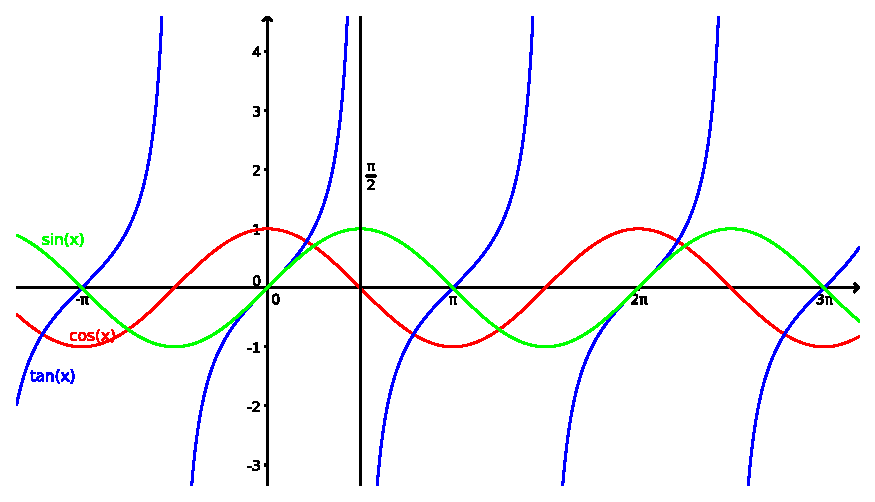
\includegraphics[width=\columnwidth]{sin_cos_tan.eps}

\subsubsection{Einheitskreis}
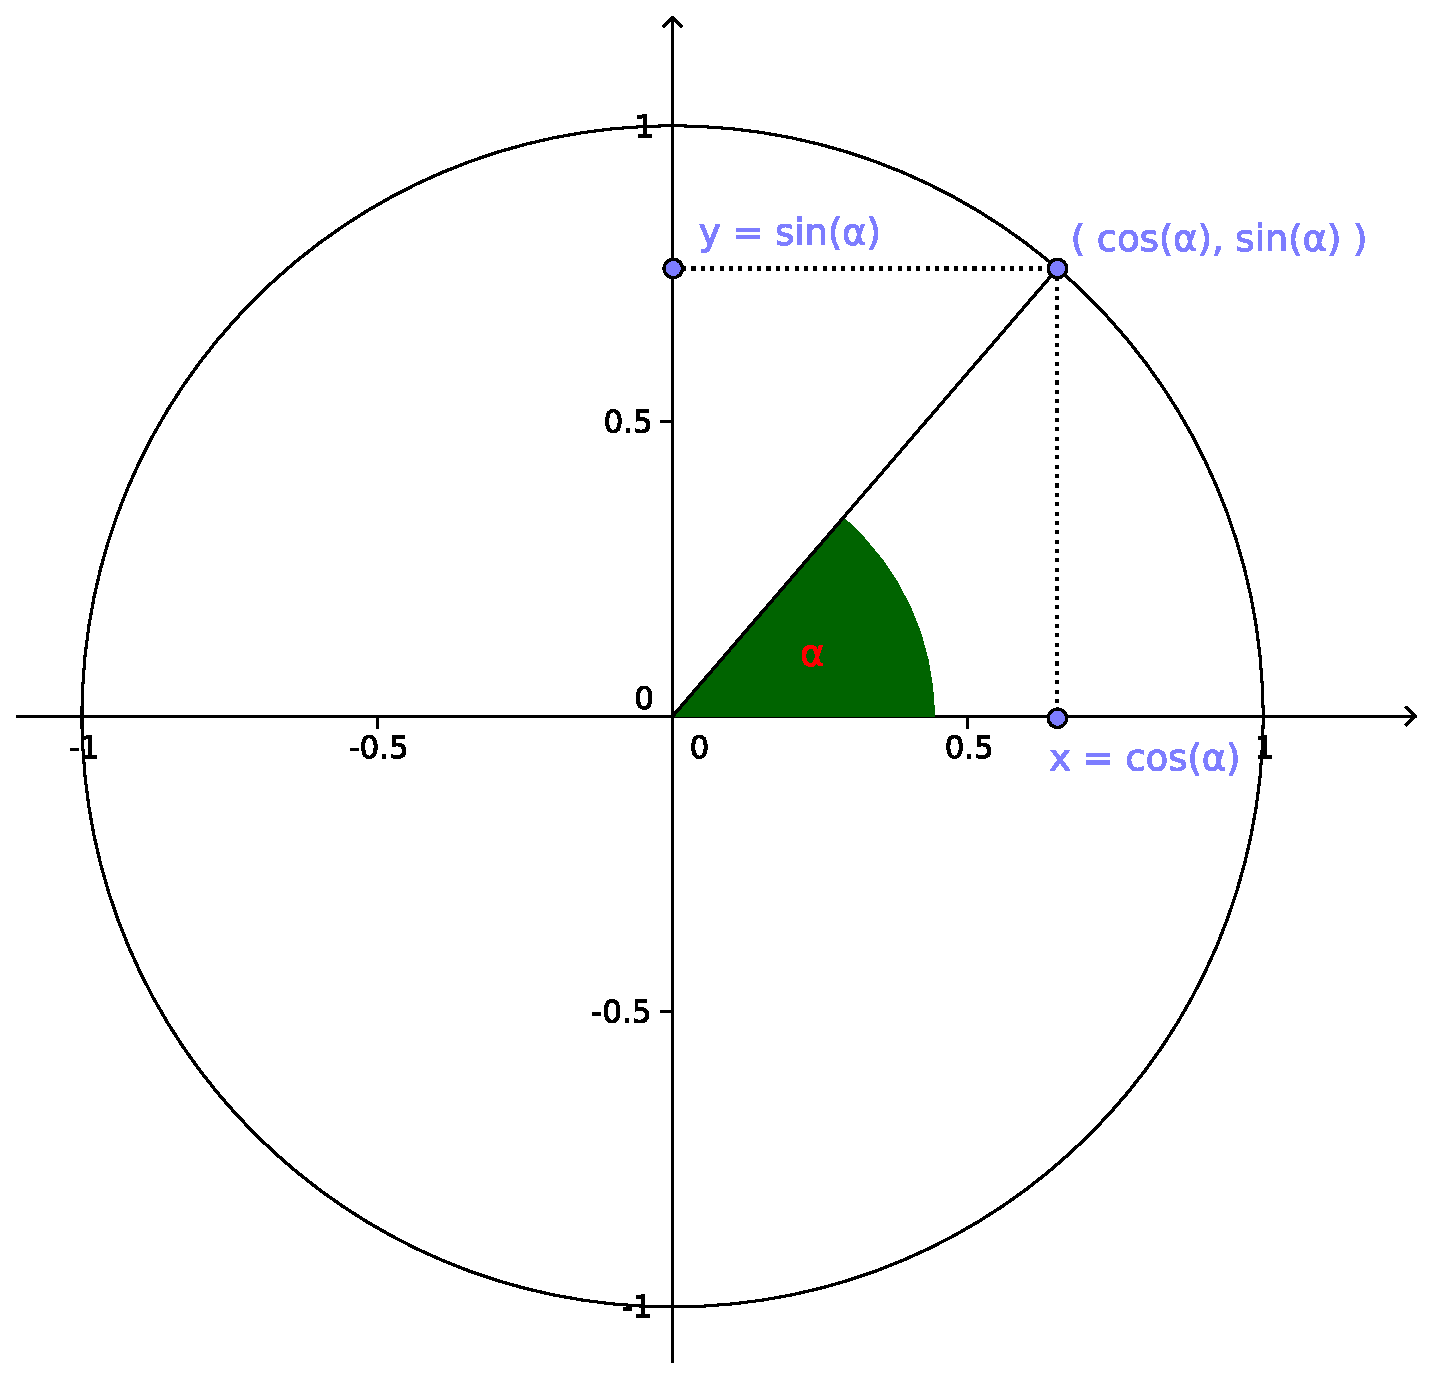
\includegraphics[width=\columnwidth]{einheitskreis_sin_cos.eps}
$\tan \alpha = \frac{\sin \alpha}{\cos \alpha} = \frac{y}{x}$

\todo{Periode für manipulierte Winkel: $\sin(0.6\alpha)$}

\subsection{Int. \& Diff. -Regeln}
\begin{itemize}[leftmargin=*]
	\item (Summenregel) $(f + g)'(x) = f'(x) + g'(x)$
	\item (Produktregel) $(fg)'(x) = f'(x)g(x) + f(x)g'(x)$
	\item (Quotientenregel) $(\frac{f}{g})'(x) = \frac{f'(x)g(x) -
	f(x)g'(x)}{g^2(x)}$
	\item (Kettenregel) $(g \circ f)'(x) = (g(f(x)))' = g'(f(x)) f'(x)$
	\item $\int u'\cdot v dx = uv - \int u \cdot v' dx$
	\item $\int f(x) dx = \int f(g(t)) g'(t) dt, \; x=g(t), dx = g'(t) dt$
\end{itemize}

\subsection{Ableitungen}
\begin{multicols}{3}
\begin{tabular}{|c|c|} \hline
$f$ & $f'$ \\\hline
$x^n$ & $n x^{n-1}$ \\
$\frac{1}{x^n}$ & $-n\frac{1}{x^{n+1}}$ \\
$\sqrt{x}$ & $\frac{1}{2 \sqrt{x}}$ \\
$\sqrt[n]{x}$ & $\frac{1}{n \sqrt[n]{x^{n-1}}}$ \\
\hline
\end{tabular}

\begin{tabular}{|c|c|} \hline
$e^x$ & $e^x$ \\
$\ln x$ & $\frac{1}{x}$ \\
$a^x$ & $a^x \ln a$ \\
$x^x$ & $x^x (1 + \ln x)$ \\
$\sin x$ & $\cos x$ \\
\hline
\end{tabular}

\begin{tabular}{|c|c|} \hline
$\cos x$ & $-\sin x$ \\
$\tan x$ & $\frac{1}{\cos^2 x}$ \\
$\arcsin x$ & $\frac{1}{\sqrt{1-x^2}}$ \\
$\arccos x$ & $-\frac{1}{\sqrt{1-x^2}}$ \\
$\arctan x$ & $\frac{1}{1 + x^2}$ \\
\hline
\end{tabular}
\end{multicols}

\subsection{Integrale}
\subsubsection{einfache Integralregeln}
Es gelte: $\int f(x) \, dx = F(x)$
\begin{itemize}[leftmargin=*]
	\item $\int f(a + x) \,dx = F(a + x)$
	\item $\int f(a - x) \,dx = -F(a-x)$
	\item $\int f(-x) \,dx = -F(-x)$
	\item $\int f(\alpha x) \,dx = \frac{1}{\alpha}F(\alpha x)$
	\item $\int \frac{g'(x)}{g(x)} \, dx = \ln|g(x)|$
	\item $\int g(x)g'(x) \, dx = \frac{1}{2}g(x)^2$
\end{itemize}
\subsubsection{typische Integrale}
\begin{itemize}[leftmargin=*]
  	\item $\int \frac{1}{x} \,dx = \ln |x|$
  	\item $\int \frac{1}{x+a} \,dx = \ln |x+a|$
  	\item $\int \frac{1}{(x+a)^2} \,dx = - \frac{1}{x+a}$
  	\item $\int \frac{1}{\sqrt{x}} \,dx = 2 \sqrt{x}$
	\item $\int \frac{1}{ax+b} \,dx = \frac{1}{a} \ln |ax+b|$
	\item $\int(ax + b)^n \,dx = \frac{(ax + b)^{n+1}}{(n + 1)a}, (n \neq -1)$
	\item $\int x(ax+b)^n \,dx = \frac{(ax + b)^{n+2}}{(n+2)a^2} -
	\frac{b(ax+b)^{n+1}}{(n+1)a^2}$
	\item $\int \frac{ax + b}{px + q} \,dx = \frac{ax}{p} + \frac{bp - aq}{p^2} \ln
	|pq+q|$
	\item $\int \frac{1}{a^2 + x^2} \,dx = \frac{1}{a} \arctan(\frac{x}{a})$
	\item $\int \frac{1}{a^2 - x^2} \,dx = \frac{1}{2a} \ln \left | \frac{a+x}{a-x}
	\right |$
	\item $\int \sqrt{x} \,dx = \frac{2}{3}\sqrt{x^3}$
\end{itemize}

\subsubsection{Integrale trionometrischer Funktionen}
\begin{itemize}[leftmargin=*]
	\item $\int \sin(ax) \,dx = -\frac{1}{a}\cos(ax)$
	\item $\int \cos(ax) \,dx = \frac{1}{a}\sin(ax)$
	\item $\int \tan(ax) \,dx = -\frac{1}{a}\log(\cos(ax))$ 
	\item $\int \sin(ax)^2 \,dx = \frac{x}{2} - \frac{sin(2ax)}{4a}$
	\item $\int \frac{1}{\sin^2 x} \,dx = -\cot x$
	\item $\int x \sin(ax) \,dx = \frac{\sin(ax)}{a^2} - \frac{x \cos(ax)}{a}$
	\item $\int \cos^2(ax) \,dx = \frac{x}{2} + \frac{\sin(2ax)}{4a}$
	\item $\int \frac{1}{\cos^2(x)} \,dx = \tan x$
	\item $\int \cos(ax) \,dx = \frac{\cos(ax)}{a^2} + \frac{x \sin(ax)}{a}$
	\item $\int \sin(ax) \cos(ax) \,dx = -\frac{sin^2(ax)}{2a}$
	\item $\int \tan(ax) \,dx = - \frac{1}{a} \ln | \cos(ax) |$
	\item $\int \arcsin(x) \,dx = x \arcsin(x) + \sqrt{1 - x^2}$
	\item $\int \arccos(x) \,dx = x \arccos(x) - \sqrt(1-x^2)$
	\item $\int \arctan(x) \,dx = x \arctan(x) - \frac{1}{2} \ln(1+x^2)$
\end{itemize}

\subsubsection{Integrale von Exponentialfunktion}
\begin{itemize}[leftmargin=*]
  	\item $\int e^{ax} \,dx = \frac{1}{a} e^{ax}$ 
	\item $\int x e^{ax} \,dx = e^{ax} \cdot \left ( \frac{ax - 1}{a^2} \right )$
	\item $\int x \ln(x) \,dx = \frac{1}{2} x^2 (\ln(x) - \frac{1}{2})$
	\item $\int_{-\infty}^\infty e^{-\frac{1}{a}x^2} \,dx = \sqrt{a \pi}$
\end{itemize}

\subsection{Trigonometrische Funktionen \& Additionstheorem}
\begin{itemize}[leftmargin=*]
	\item $\sin^2(x) + \cos^2(x) = 1$
	\item $\frac{1}{\cos^2(\alpha)} = 1 + \tan^2(\alpha)$
	\item $\sin(90^\circ \pm \alpha) = \cos(\alpha)$
	\item $\sin(180^\circ \pm \alpha) = \mp \sin(\alpha)$
	\item $\cos(90^\circ \pm \alpha) = \mp \sin(\alpha)$
	\item $\cos(180^\circ \pm \alpha) = - \cos(\alpha)$
	\item $\sin(\alpha \pm \beta) = \sin(\alpha)\cos(\beta) \pm
	\cos(\alpha)\sin(\beta)$
	\item $\cos(\alpha \pm \beta) = \cos(\alpha)\cos(\beta) \mp \sin(\alpha)
	\sin(\beta)$
	\item $\tan(\alpha \pm \beta) = \frac{\tan(\alpha) \pm \tan(\beta)}{1 \mp
	\tan(\alpha)\tan(\beta)}$
	\item $\sin(2\alpha) = 2 \sin(\alpha)\cos(\alpha)$
	\item $\cos(2\alpha) = \cos^2(\alpha) - \sin^2(\alpha) = 2 \cos^2(\alpha) - 1
	= 1 - 2 \sin^2(\alpha)$
	\item $\tan(2\alpha) = \frac{2 \tan(\alpha)}{1 - \tan^2(\alpha)}$
\end{itemize}

\subsection{Reihenentwicklung}
\begin{itemize}[leftmargin=*]
	\item $e^x = \sum_{n=0}^\infty \frac{x^n}{n!} = 1 + \frac{x}{1!} +
	\frac{x^2}{2!} + \cdots$
	\item $\sin x = \sum_{n=0}^\infty (-1)^n \frac{x^{2n + 1}}{(2n + 1)!} = x -
	\frac{x^3}{3!} + \frac{x^2}{5!} + \cdots$
	\item $\cos x = \sum_{n=0}^\infty (-1)^n \frac{x^{2n}}{(2n)!} = 1 -
	\frac{x^2}{2!} + \frac{x^4}{4!} - \cdots + \cdots$
	\item $\sinh x = \sum_{n=0}^\infty \frac{x^{2n+1}}{(2n + 1)!}$
	\item $\cosh x = \sum_{n=0}^\infty \frac{x^{2n}}{(2n)!}$
	\item $\ln x = \sum_{n=0}^\infty \frac{2}{2n + 1} \cdot \left(
	\frac{x-1}{x+1} \right)^{2n}$
\end{itemize}

\subsection{Grenzwerte}
\begin{itemize}[leftmargin=*]
	\item \textbf{Bernoullische Ungleichung}: $x \geq -1, n \in \N: \; (1+x)^n \geq
	1+nx$
	\item \textbf{Vergleich von Folgen}: weiter rechts stehende Folgen streben
	schneller gegen $\infty$ als die links davon stehenden: $1, \quad \ln n, \quad
	n^\alpha (\alpha > 0), \quad q^n (q > 1), \quad n!, \quad n^n$ $\Rightarrow
	\lim_{x \to \infty} \frac{\ln n}{n^\alpha} = 0$
\end{itemize}
\subsubsection{$x \rightarrow \infty$}
\begin{multicols}{2}
\begin{itemize}[leftmargin=*]
	\item $\sqrt[n]{a} \rightarrow 1$
	\item $\sqrt[n]{n} \rightarrow 1$
	\item $\sqrt[n]{n!} \rightarrow \infty$
	\item $\frac{n}{\sqrt[n]{n!}} \rightarrow e$
	\item $\frac{1}{n} \sqrt[n]{n!} \rightarrow \frac{1}{e}$
	\item $\left ( \frac{n+1}{n} \right )^n \rightarrow e$
	\item $\left ( 1 + \frac{1}{n} \right )^n \rightarrow e$
	\item $\left ( 1 - \frac{1}{n} \right )^n \rightarrow \frac{1}{e}$
	\item $\left ( 1 + \frac{x}{n} \right )^n \rightarrow e^x$
	\item $\left ( 1 - \frac{x}{n} \right )^n \rightarrow \frac{1}{e^x}$
	\item ${a \choose n} \rightarrow 0, \; a > -1$
	\item $\frac{a^n}{n!} \rightarrow 0$
	\item $\frac{n^n}{n!} \rightarrow \infty$
	\item $\frac{a^n}{n^k} \rightarrow \infty, a > 1, k$ fest
	\item $a^n n^k \rightarrow 0, |a| < 1, k$ fest
	\item $n(\sqrt[n]{a} - 1) \rightarrow \ln a, a > 0$
\end{itemize}
\end{multicols}
\subsubsection{$x \to 0$}
\begin{multicols}{2}
\begin{itemize}[leftmargin=*]
  \item $\frac{a^x - 1}{x} = \ln a$
  \item $\frac{\sin x}{x} = 1$
  \item $\frac{1 - \cos x}{x} = 0$
  \item $\frac{\log_a (1 + x)}{x} = \frac{1}{\ln a}$
  \item $x^a \ln x = 0, \; a  > 0$
\end{itemize}
\end{multicols}

\subsection{Reihen}
\begin{itemize}[leftmargin=*]
	\item $\sum_{n=1}^\infty \frac{1}{n}$ divergiert (``harmonische Reihe'')
	\item $\sum_{n=1}^\infty \frac{(-1)^n}{n} = \ln \frac{1}{2}$
	\item $\sum_{n=1}^\infty \frac{1}{n^\alpha}$ konvergiert für $\alpha > 1$,
	divergiert für $\alpha \leq 1$
	\item $\sum_{n=1}^m n = \frac{m(m+1)}{2}$
	\item $\sum_{n=0}^\infty q^n = \frac{1}{1-q}$ für $|q| < 1$ (``geometrische
	Reihe'')
	\item $\sum_{n=1}^\infty \frac{1}{n^2} = \frac{\pi^2}{6}$
	\item $\sum_{n=0}^m q^n = \frac{1-q^{m+1}}{1-q}$ 
\end{itemize}

\subsection{\texorpdfstring{$\log(x)$}{log(x)}}
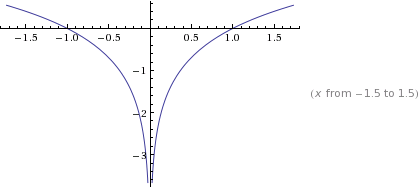
\includegraphics[scale=0.5]{log_x.png}

\subsection{\texorpdfstring{$\frac{1}{x}$}{1/x}}
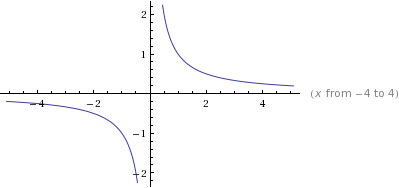
\includegraphics[scale=0.5]{1_over_x.png}

\subsection{\texorpdfstring{$\sqrt{x}$}{x^(1/x)}}
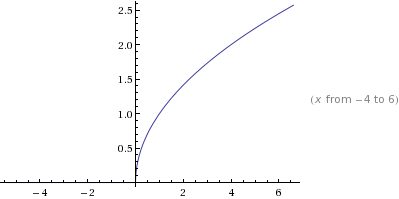
\includegraphics[scale=0.5]{sqrt_x.png}

\subsection{Kreuzprodukt}
{\footnotesize
\[
\vec{a} \times \vec{b} = \left ( \begin{array}{c} a_1 \\ a_2 \\ a_3 \end{array}
\right ) \times
\left ( \begin{array}{c} b_1 \\ b_2 \\ b_3 \end{array}
\right ) =
\left ( \begin{array}{c} a_2b_3 - a_3b_2 \\ a_3b_1 - a_1b_3 \\ a_1b_2 - a_2b_1
\end{array} \right )
\]
}

\subsection{Geometrische Körper}
\subsubsection{Ellipsoid}
Hat die Form eines Rugbyballs. In kartesischen Koordinaten definert durch
$\frac{x^2}{a^2} + \frac{y^2}{b^2} + \frac{z^2}{c^2} - 1 = 0$.

\subsection{Ausklammern}
\begin{itemize}[leftmargin=*]
	\item $x^n - y^n = (x-y) (x^{n-1} + x^{n-2}y + x^{n-3}y^2 + \ldots + xy^{n-2}
	+ y^{n-1})$
	\item $x^n - 1 = (x-1)(x^{n-1} + x^{n-2} + \ldots + x + 1)$
\end{itemize}

\subsection{Aus Serien}
\begin{itemize}[leftmargin=*]
	\item Ableitung von $x^x$ kann man berechnen, indem man $x = e^{\log(x)}$
	setzt. Also in diesem Fall $e^{\log(x^x)} = e^{x \log(x)}$ ableitet, was $e^{x
	\log(x)} (1 + \log(x))$ (Serie 10)
	\item Cauchy-Schwarz Ungleichung: $|x \cdot y| \leq \|x\| \cdot \|y\|, \; x,y \in \R^n$
\end{itemize}

\subsection{Funktionsmanipulation}
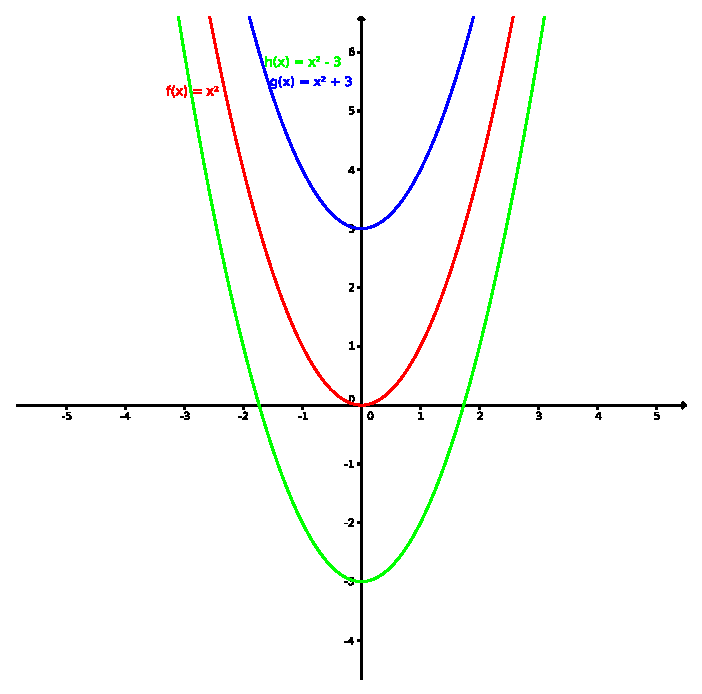
\includegraphics[width=\columnwidth]{manipulation_1.eps}
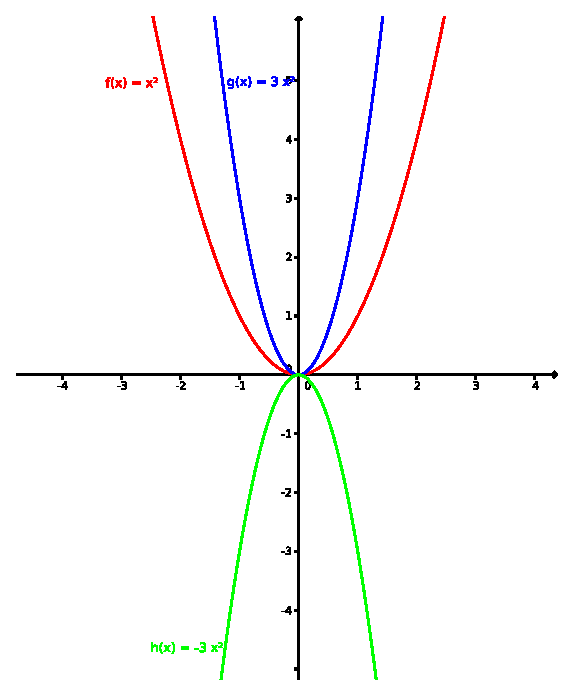
\includegraphics[width=\columnwidth]{manipulation_2.eps}
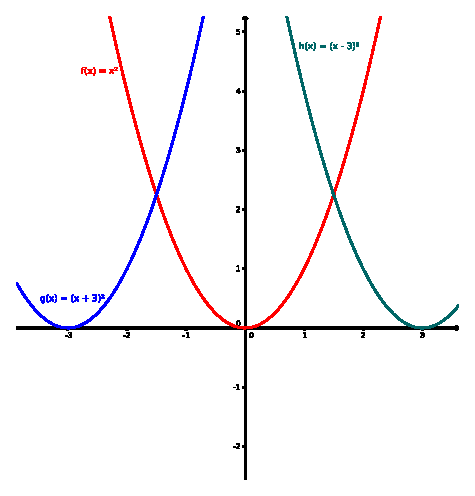
\includegraphics[width=\columnwidth]{manipulation_3.eps}

\begin{multicols}{2}

\subsection{Exponent}
\begin{itemize}[leftmargin=*]
  \item $a^n a^m = a^{n + m}$
  \item $(a^n)^m = a^{nm}$
  \item $(ab)^n = a^n b^n$
  \item $\left( \frac{a}{b} \right)^n = \frac{a^n}{b^n}$
  \item $a^{-n} = \frac{1}{a^n}$
  \item $\left( \frac{a}{b} \right)^{-n} = \left( \frac{b}{a} \right)^n$
  \item $a^\frac{n}{m} = (a^\frac{1}{m})^n = (a^n)^\frac{1}{m}$
\end{itemize}
\columnbreak

\subsection{Wurzel}
\begin{itemize}[leftmargin=*]
  \item $\sqrt[n]{a} = a^\frac{1}{n}$
  \item $\sqrt[n]{ab} = \sqrt[n]{a} \sqrt[n]{b}$
  \item $\sqrt[m]{\sqrt[n]{a}} = \sqrt[nm]{a}$
  \item $\sqrt[n]{\frac{a}{b}} = \frac{\sqrt[n]{a}}{\sqrt[n]{b}}$
\end{itemize}

\end{multicols}

\subsection{Ungleichungen}
\begin{itemize}[leftmargin=*]
  \item $a < b \Rightarrow a + c < b + c$ und $a - c < b - c$
  \item $a < b$ und $c > 0 \Rightarrow \frac{a}{c} < \frac{b}{c}$
  \item $a < b$ und $c < 0 \Rightarrow \frac{a}{c} > \frac{b}{c}$ 
\end{itemize}

\subsection{Logarithmen}
\begin{itemize}[leftmargin=*]
  \item $y = \log_a x \Leftrightarrow x = a^y$
  \item $\log_a 1 = 0$
  \item $\log_a a^x = x$
  \item $a^{\log_a x} = x $
  \item $\log_a xy = \log_a x + \log_a y$
  \item $\log_a \frac{1}{x} = - \log_a x$
  \item $\log_a x^r = r \log_a x$
  \item $\log_a x = \frac{\log_b x}{\log_b a}$
  \item $\log_a x = \frac{\ln x}{\ln a}$
  \item $\log_a (x+y) = \log_a x + log_a (1 + \frac{y}{x})$
  \item $\log_a (x-y) = \log_a x + \log_a (1- \frac{y}{x})$
\end{itemize}

